%%%%%%%%%%%%%%%%%%%%%%%%%%%%%%%%%%%%%%%%%%%%%%%%%%%%%%%%%%%%%%%%%%%%%%%%%%%%%
\section{Examples of OpencCL Applications}


%------------------------------------------------------------------------------
\subsection{OpenCL on FPGA platforms}

\subsubsection{OpenCL-FPGA Implementation}
As we already saw, OpenCL applications consists of two part: the host and the kernels.
FPGA flexibility allow the developer to opt for two solutions:

\begin{enumerate}
	\item An "`All in One"' solution, by implementing the CPU that will run the standard C/C++ host code directly as a soft CPU inside the FPGA.
	\item A separate solution, by using an external microprocessor for the host and by programming the FPGA to execute the kernels only.
	\end{enumerate}
	
Unlike CPUs and GPUs, where parallel threads can be executed on different cores, FPGAs offer a different strategy. Kernel functions can be transformed into dedicated and deeply pipelined \textbf{hardware circuits} that are inherently multithreaded using the concept of pipeline parallelism. Each of these pipelines can be replicated many times to provide even more parallelism than is possible with a single pipeline. This translates in an immediate boost in performance.\\
Figure \ref {fig:fpga_example} shows a simple example of how kernels are translated into separate \textbf{hardware pipelines}.
	
\begin{figurehere}
 \centering
 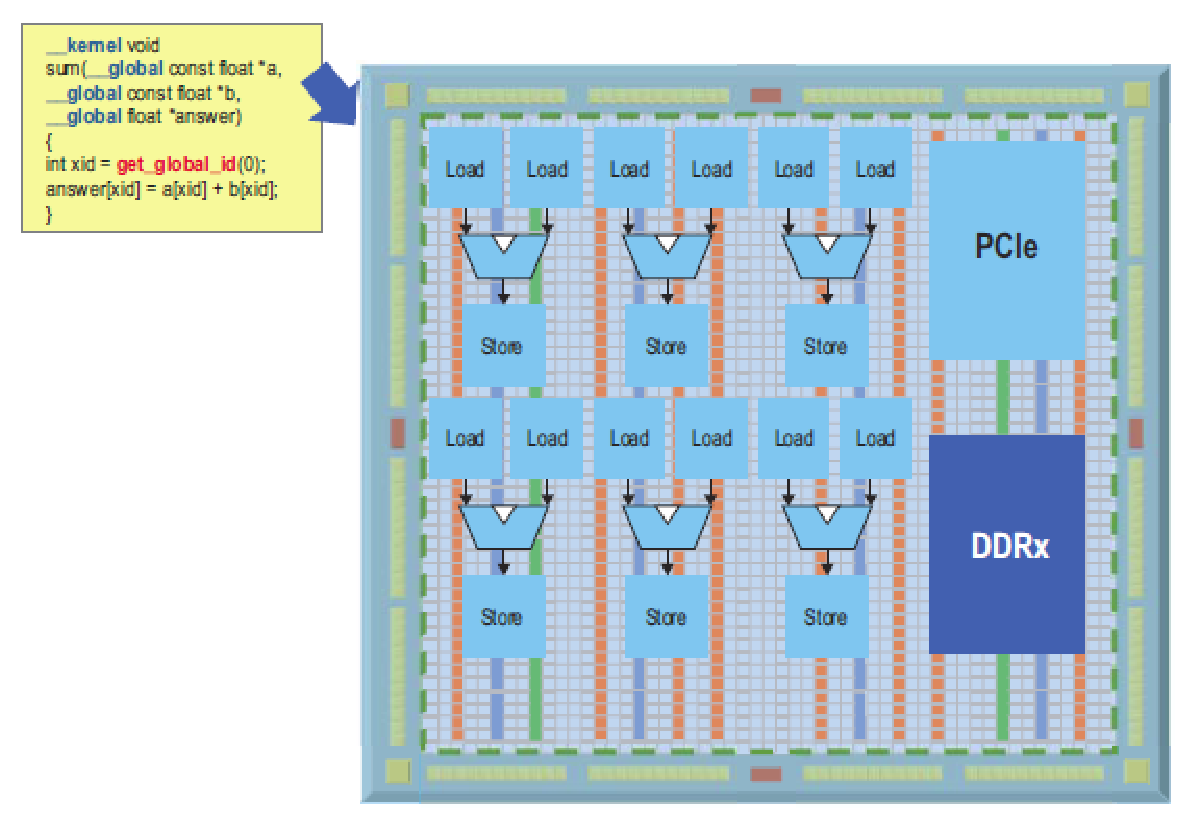
\includegraphics[width=8cm, height=4cm]{./eps/FPGA1.eps}
 \caption{FPGA implementation example}
 \label{fig:fpga_example}
\end{figurehere}

The most important concept behind the OpenCL-to-FPGA compiler is the notion of \textbf{pipeline parallelism}.
Basically, an OpenCL-to-FPGA compiler is able to implement the scenario observed in Section \ref{sect:pipelineScenario} in an automatic and more efficient way. We will describe how pipeline parallelism work by introducing an example, shown in Figure \ref{fig:fpga_example2}:

\begin{figurehere}
 \centering
 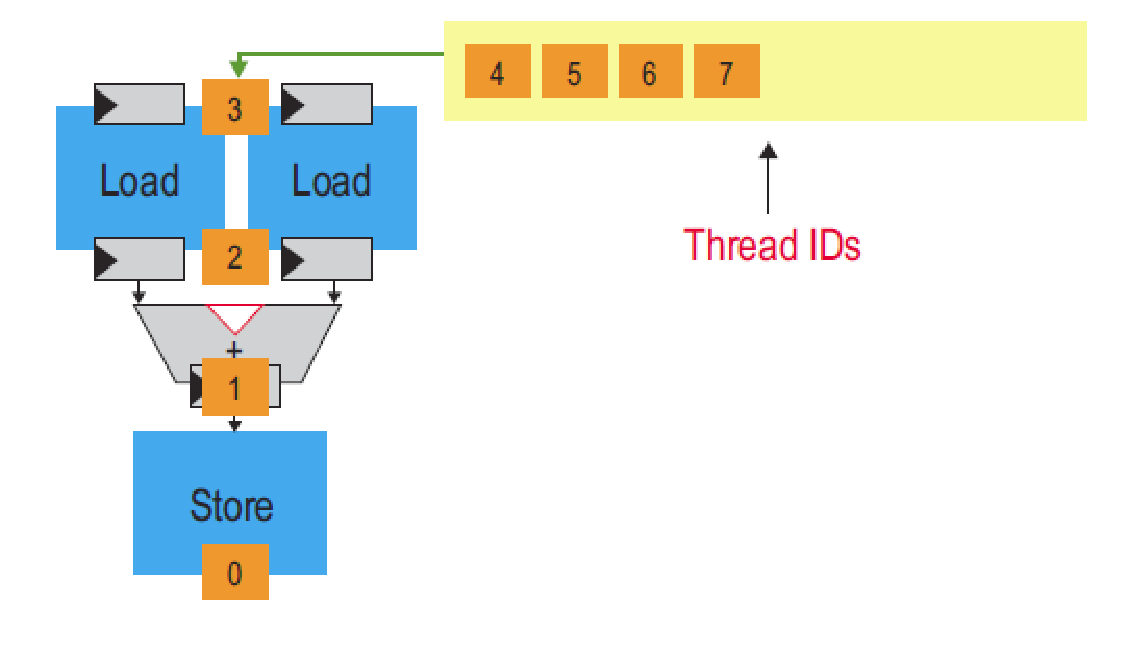
\includegraphics[width=8cm, height=4cm]{./eps/FPGA2.eps}
 \caption{Pipeline parallelism example}
 \label{fig:fpga_example2}
\end{figurehere}

On the first clock cycle, thread 0 is clocked into the two load units. This indicates that they should begin fetching the first elements of data from arrays A and B. On the second clock cycle, thread 1 is clocked in
at the same time that thread 0 has completed its read from memory and stored the results in the registers following the load units. On cycle 3, thread 2 is clocked in, thread 1 captures its returned data, and thread 0 stores the sum of the two values that it loaded. It is evident that in the steady state, all parts of the pipeline are active, with each stage processing a different thread.
	
To complete this section, we'll present a general scheme that summarize how OpenCL-FPGA applications are implemented (Figure \ref{fig:fpga_implementation}). One crucial point for parallel computation is the memory management, and as we can see from the figure several memory interfaces are needed, but luckily OpenCL-FPGA compilers are usually able to implement such interfaces automatically.

\begin{figurehere}
 \centering
 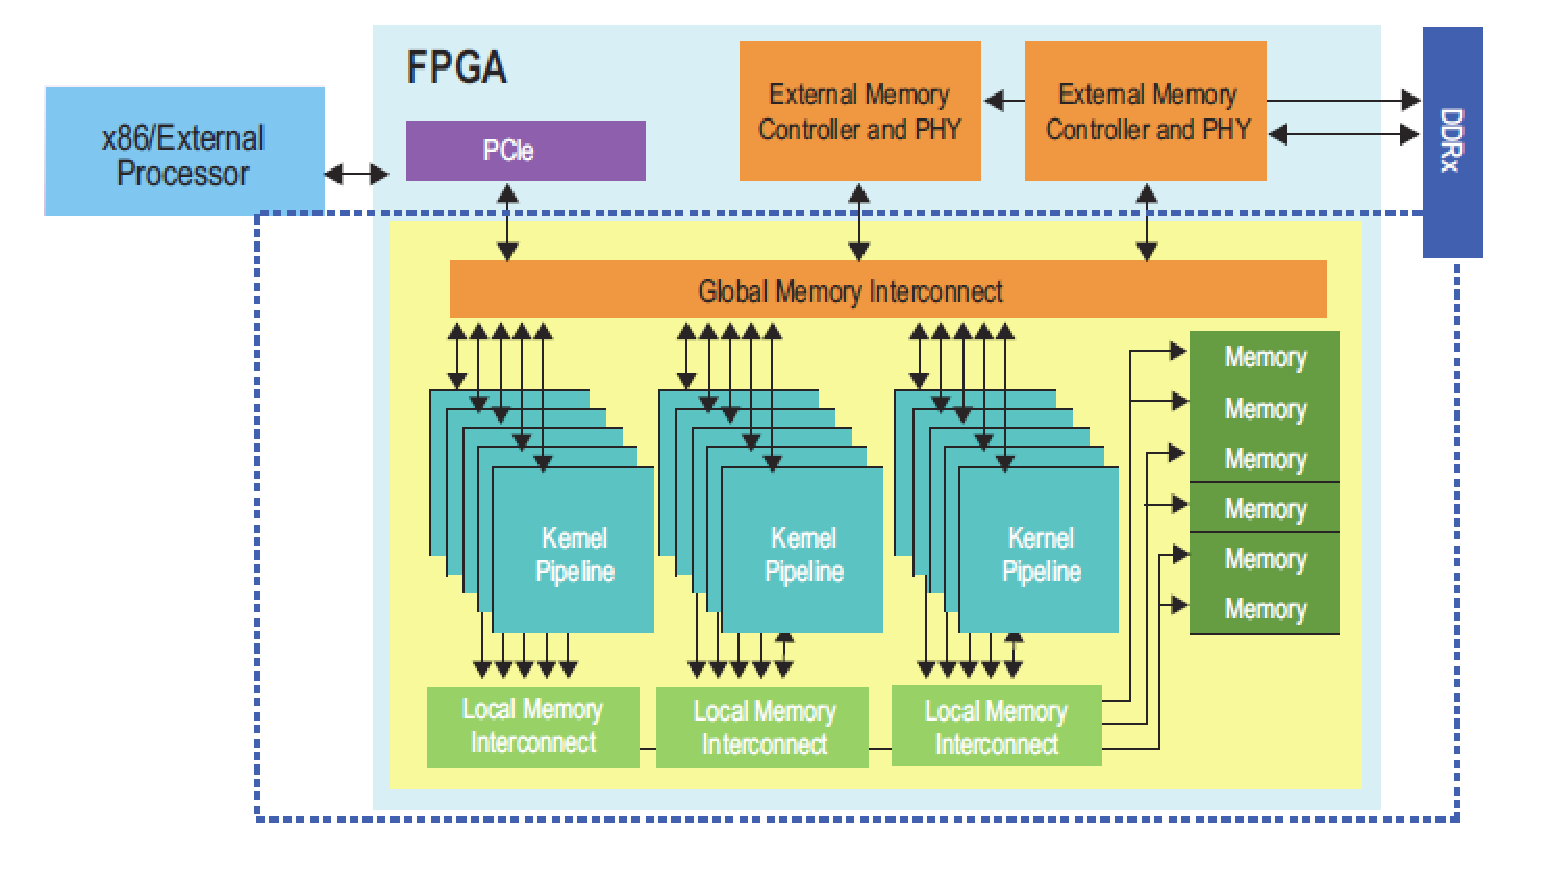
\includegraphics[width=8cm, height=4cm]{./eps/FPGA3.eps}
 \caption{OpenCL-FPGA Implementation scheme}
 \label{fig:fpga_implementation}
\end{figurehere}

\subsubsection{Benefits}

\begin{itemize}
	\item \textbf{Improved Time To Market:} OpenCL offers a quicker and simpler way to implement parallel alghorithms  compared to traditional FPGA development using lower level hardware description language (HDLs) such as Verilog or VHDL \cite {altera:FPGA}.  This because OpenCL inherently offers the ability to describe parallel computation, while the main challenge in HDLs languages was exactly to extract thread-level parallelism from a sequential program. OpenCL offers instead the ability to the programmer to explicitly specify and control parallelism.
	\item \textbf{Better Performance:} Dedicated ad-hoc hardware structures allow faster computation than using generic CPUs. Furthermore OpenCL-FPGA compilers exploit pipeline parallelism to make computation even faster.
	\item \textbf{Less Power Consumption:} Benchmarks show that FPGA applications consumes lot less power to execute the same OpenCL code in comparison to CPU or GPU.
\end{itemize}

\subsubsection{Case Study: Monte Carlo Black-Scholes Method}

In this experiment an economic model was used to benchmark an OpenCL-FPGA unit. The model is based on the 
Monte Carlo Black-Scholes method and it is used to compute the expected payoff of stock prices over millions of different paths. The entire algorithm used for this benchmark can be implemented in approximately 300 lines of
OpenCL code that is portable from FPGA to CPU to GPU, and we can see the comparison in performance on these 3 different platforms in Table \ref{tab:FPGABenchmark}.

\begin{tablehere}
{\footnotesize
\begin{tabular}{|p{1,0cm}|p{1,8cm}|p{1,8cm}|p{1,8cm}|}\hline
\textbf{Platform} & \textbf{Power} [Watts] & \textbf{Performance} [Billions of simulations per seconds] & \textbf{Efficiency} [Millions of sims per second per watt]\\ \hline
CPU & 130 & 0.032 & 0.0025 \\ \hline
GPU & 212 & 10.1 & 48 \\ \hline
FPGA & 45 & 12.0 & 266 \\ \hline
\end{tabular}}
  \caption{Monte Carlo Black-Scholes benchmark results\\}
	\label{tab:FPGABenchmark}
\end{tablehere}

As we can see, not only the OpenCL framework targeting a FPGA board exceeds the throughput of both a CPU and a GPU, but it also consumes one-fifth the power of comparable GPUs when executing the same code.

\subsubsection{Case Study: Document Filtering}

In this benchmark the focus is set on a more practical problem than the previous, as it will consider an algorithm used in modern data centers.
A recent report \cite{walsh:power} from International Data Corporation (IDC) examined the requirements of high performance computing data centers, and conducted a survey of the top constraints in expanding current data center capabilities. From the results, it was obvious that power and cooling costs are the key impediments of compute capability expansion, and as we have seen in the previous benchmark, FPGA computation offer an huge improvement in power consumption over CPUs and GPUs.\\

In this experiment, a document filtering algorithm was implemented using OpenCl, and it basically involves looking at an incoming stream of documents and finding the ones that best match a user’s interest. The results are shown in Table \ref{tab:FPGABenchmark2}:

\begin{tablehere}
{\footnotesize
\begin{tabular}{|p{1,0cm}|p{1,8cm}|p{1,8cm}|p{1,8cm}|}\hline
\textbf{Platform} & \textbf{Power} [Watts] & \textbf{Performance} [Million of Terms per seconds] & \textbf{Efficiency} [Millions of Terms per Joule]\\ \hline
CPU & 130** & 2070 & 15.9 \\ \hline
GPU & 215 & 3240 & 15.1 \\ \hline
FPGA & 21 & 1755 & 83.6 \\ \hline
\end{tabular}}
  \caption{Document Filtering benchmark results\\ **Does not include memory consumption.}
	\label{tab:FPGABenchmark2}
\end{tablehere}

As we can see, although CPUs and GPUs can perform better in terms on throughput, the power efficiency of these two platform can be five time lower than the efficiency of FPGAs. It is interesting to note that in this case the performance of the FPGA was limited by the external memory bandwidth, and not by the FPGA itself. With a proper setup, the authors extimate a performance value of 2925 MT/s with the same power consumption, that would raise the power efficiency from 83.6 MT/J to 139,3 MT/J.
These results demonstrate that introducing an FPGA OpenCL implementation of algorithms, could bring a dramatic decrease of power consumption and thus cooling costs in modern data centers.


%-----------------------------------------------------------------------------



